\documentclass{article}
\usepackage{multicol}
\usepackage{tikz}

\title{{Propositional Logic}}

\begin{document}
\maketitle

\begin{center}
  \rule{0.5\textwidth}{0.4pt}
\end{center}

\section{Propositions}
\begin{itemize}
  \item{A \textbf{\textit{Proposition}} is an atomic statement that either has the truth value $true$ or $false$}
  \item{For example:}
  \begin{itemize}
    \item{$1 + 1 = 2$}
    \item{$1 + 2 = 4$}
    \item{The Earth is closer to the Sun than Mars}
    \item{My eyes are green}
  \end{itemize}
\end{itemize}

\begin{center}
  \rule{0.5\textwidth}{0.4pt}
\end{center}

\section{Boolean Operators}
\begin{itemize}
  \item{Negation}
  \begin{itemize}
    \item{\textbf{\textit{Negation}} is a unary boolean operator}
    \item{This means it only takes one arugment}
    \item{The truth table for negation is:} \\
    \begin{center}
      \begin{tabular}{ |c|c| }
        \hline
        $x$ & $\neg{x}$ \\
        \hline
        $true$ & $false$ \\
        $false$ & $true$ \\
        \hline
      \end{tabular}
    \end{center}
  \end{itemize}
  \pagebreak
  \item{Conjunction}
  \begin{itemize}
    \item{\textbf{\textit{Conjunction}} is a binary boolean operator}
    \item{This means it takes two arguments}
    \item{The truth table for conjunction is:} \\
    \begin{center}
      \begin{tabular}{ |c|c|c| }
        \hline
        $x$ & $y$ & $x \land y$ \\
        \hline
        $false$ & $false$ & $false$ \\
        $false$ & $true$ & $false$ \\
        $true$ & $false$ & $false$ \\
        $true$ & $true$ & $true$ \\
        \hline
      \end{tabular}
    \end{center}
  \end{itemize}
  \item{Disjunction}
  \begin{itemize}
    \item{\textbf{\textit{Disjunction}} is a binary boolean operator}
    \item{This is the truth table for disjunction:} \\
    \begin{center}
      \begin{tabular}{ |c|c|c| }
        \hline
        $x$ & $y$ & $x \lor y$ \\
        \hline
        $false$ & $false$ & $false$ \\
        $false$ & $true$ & $true$ \\
        $true$ & $false$ & $true$ \\
        $true$ & $true$ & $true$ \\
        \hline
      \end{tabular}
    \end{center}
  \end{itemize}
  \item{Exclusive-Or}
  \begin{itemize}
    \item{\textbf{\textit{Exclusive-or}} is a binary boolean operator}
    \item{This is the truth table for exclusive-or} \\
    \begin{center}
      \begin{tabular}{ |c|c|c| }
        \hline
        $x$ & $y$ & $x \oplus y$ \\
        \hline
        $false$ & $false$ & $false$ \\
        $false$ & $true$ & $true$ \\
        $true$ & $false$ & $true$ \\
        $true$ & $true$ & $false$ \\
        \hline
      \end{tabular}
    \end{center}
  \end{itemize}
  \item{Implication}
  \begin{itemize}
    \item{\textbf{\textit{Impication}} is a binary boolean operator}
    \item{$x \Rightarrow y$ means that when $x$ when is $true$, $y$ is $true$, but $y$ can be $true$ when $x$ is false}
    \item{This is the truth table for implication}
    \begin{center}
      \begin{tabular}{ |c|c|c| }
        \hline
        $x$ & $y$ & $x \Rightarrow y$ \\
        \hline
        $false$ & $false$ & $true$ \\
        $false$ & $true$ & $true$ \\
        $true$ & $false$ & $false$ \\
        $true$ & $true$ & $true$ \\
        \hline
      \end{tabular}
    \end{center}
  \end{itemize}
  \item{Equivalence}
  \begin{itemize}
    \item{\textbf{\textit{Equivalence}} is a binary boolean operator}
    \item{This is the truth table for equivalence} \\
    \begin{center}
      \begin{tabular}{ |c|c|c| }
        \hline
        $x$ & $y$ & $x \Leftrightarrow y$ \\
        \hline
        $false$ & $false$ & $true$ \\
        $false$ & $true$ & $false$ \\
        $true$ & $false$ & $false$ \\
        $true$ & $true$ & $true$ \\
        \hline
      \end{tabular}
    \end{center}
  \end{itemize}
  \item{Nand}
  \begin{itemize}
    \item{\textbf{\textit{Nand}} is a binary boolean operator}
    \item{It is the negation of conjunction}
    \item{This is the truth table for nand} \\
    \begin{center}
      \begin{tabular}{ |c|c|c| }
        \hline
        $x$ & $y$ & $x \Uparrow y$ \\
        \hline
        $false$ & $false$ & $true$ \\
        $false$ & $true$ & $true$ \\
        $true$ & $false$ & $true$ \\
        $true$ & $true$ & $false$ \\
        \hline
      \end{tabular}
    \end{center}
  \end{itemize}
  \item{Nor}
  \begin{itemize}
    \item{\textbf{\textit{Nor}} is a binary boolean operator}
    \item{It is the negation of disjunction}
    \item{This is the truth table for nor} \\
    \begin{center}
      \begin{tabular}{ |c|c|c| }
        \hline
        $x$ & $y$ & $x \Downarrow y$ \\
        \hline
        $false$ & $false$ & $true$ \\
        $false$ & $true$ & $true$ \\
        $true$ & $false$ & $true$ \\
        $true$ & $true$ & $false$ \\
        \hline
      \end{tabular}
    \end{center}
  \end{itemize}
\end{itemize}

\begin{center}
  \rule{0.5\textwidth}{0.4pt}
\end{center}
\pagebreak

\section{Boolean Formulae}
\begin{itemize}
  \item{if $P$ is the set of atomic propositions, a boolean formula $bf$ can be derived from the following rules:}
  \begin{itemize}
    \item{$bf ::= p$ \textit{where} $p \in P$}
    \item{$bf ::= \neg{bf}$}
    \item{$bf ::= bf$ $op$ $bf$}
    \item{$op ::= \land|\lor|\oplus|\Rightarrow|\Leftarrow|\Leftrightarrow|\Uparrow|\Downarrow$}
  \end{itemize}
  \item{We will denote the set of boolean formulae defined by the above rule as $F$}
\end{itemize}

\begin{center}
  \rule{0.5\textwidth}{0.4pt}
\end{center}

\section{Ambiguity, Precendence and Associativity}
\begin{itemize}
  \item{The previous rules by themselves are not sufficient to assign a single meaning to the following formula}
  \begin{center}
  $p \Rightarrow q \Leftrightarrow \neg{p} \Leftrightarrow \neg{q}$
  \end{center}
  \setlength{\columnsep}{0.3\textwidth}
  \begin{multicols}{2}
    [We can represent this formula by at least two different trees]
    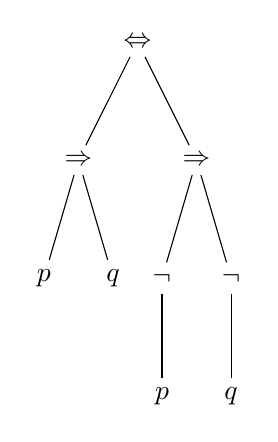
\begin{tikzpicture}
    \tikzstyle{level 2}=[sibling distance=2.5em]
      \node {$\Leftrightarrow$}
        child { node {$\Rightarrow$}
          child { node {$p$} }
          child { node {$q$} }}
        child { node {$\Rightarrow$}
          child { node {$\neg$}
            child { node {$p$} }}
          child { node {$\neg$}
            child { node {$q$} }}};
    \end{tikzpicture}
    \begin{tikzpicture}
      \node {$\Rightarrow$}
        child { node {$q$} }
        child { node {$\Leftrightarrow$}
          child { node {$q$}}
          child { node {$\neg$}
            child { node {$\Rightarrow$}
              child { node {$q$}}
              child { node {$\neg$}
                child { node {$q$}}}}} };
    \end{tikzpicture}
  \end{multicols}
  \item{When the same formula can have more than one meaning, the formula is \textit{ambiguous}}
  \item{Ambiguity can be addressed by:}
  \begin{itemize}
    \item{Using parentheses}
    \item{Assigning \textit{precedence} to the operators}
    \item{assuming that operators \textit{associate} from left to right}
  \end{itemize}
  \item{The order of \textit{precedence} from highest to lowest it:}
  \begin{center}
  $\neg$ \\ $\lor$,$\Uparrow$ \\ $\land$,$\Downarrow$ \\ $\Rightarrow$ \\ $\Leftrightarrow$,$\oplus$ \\
  \end{center}
  \begin{multicols}{2}
  [So, now we have only one meaning for each of the following formulae]
  $p \Rightarrow q \Leftrightarrow \neg{p} \Rightarrow \neg{q}$
  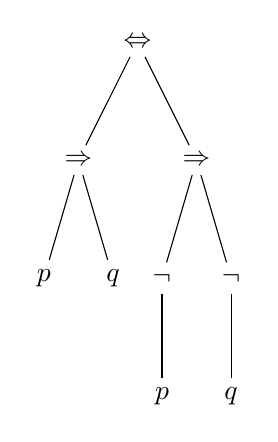
\begin{tikzpicture}
  \tikzstyle{level 2}=[sibling distance=2.5em]
    \node {$\Leftrightarrow$}
      child { node {$\Rightarrow$}
        child { node {$p$}}
        child { node {$q$}}}
      child { node {$\Rightarrow$}
        child { node {$\neg$}
          child { node {$p$}}}
        child { node {$\neg$}
          child {node {$q$}}}};
  \end{tikzpicture} \\
  \columnbreak
  $p \Rightarrow (q \Leftrightarrow \neg{(p \Rightarrow \neg{q})})$
  \begin{tikzpicture}
    \node {$\Rightarrow$}
      child { node {$p$}}
      child { node {$\Leftrightarrow$}
        child { node {$q$}}
        child { node {$\neg$}
          child { node {$\Rightarrow$}
            child { node {$p$}}
            child { node {$\neg$}
              child { node {$q$}}}}}};
  \end{tikzpicture}
  \end{multicols}
\end{itemize}

\end{document}
